% This is auto-generated file: do not edit!
% Exported from microMathematics Plus, version 2.22.1


Este ejemplo demuestra cómo preparar y
ajustar una representación gráfica de
una función. por ejemplo, queremos
trazar tres diferentes funciones:
\begin{center}\begin{tabular}{c}
  $f(x) := 25 + 10 \cdot sin \left( \sqrt{ \left| x \right| } \right) $
\end{tabular}\end{center}
\begin{center}\begin{tabular}{c}
  $g(x) := \frac{2}{{e}^{ \left| x \right|  / 15}} \cdot f \left( x \cdot 50\right) $
\end{tabular}\end{center}
\begin{center}\begin{tabular}{c}
  $h(x) := min \left( f \left( x\right) ,\, g \left( x\right) \right) $
\end{tabular}\end{center}

El argumento de la función que
representa los valores x se tomarán
para puntos N dentro del intervalo
[x1, x2]:
\begin{center}\begin{tabular}{ccc}
  $N := 300$ &
  $x1 := -30$ &
  $x2 := 30$ \cr
\end{tabular}\end{center}
\begin{center}\begin{tabular}{c}
  $x := \left[ x1,\, x1 + \left( x2 - x1 \right) / N \,..\, x2 \right]$
\end{tabular}\end{center}

Una vez definidas las funciones y sus
argumentos se puede añadir el cuadro
de trazado mediante el botón ''Nuevo
elemento'' de la barra de acciones o el
botón ''Añadir gráfico de función'' de
la barra de herramientas:
\begin{center}\begin{tabular}{c} 
\includegraphics[width=0.45\textwidth]{graphics/function_plot_fig1.png} \end{tabular}\end{center}
\begin{center}\begin{tabular}{c} 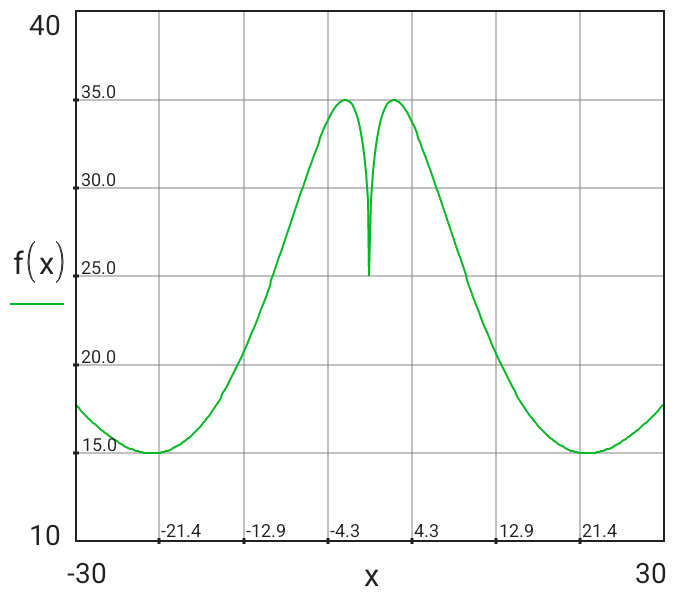
\includegraphics[width=0.45\textwidth]{graphics/function_plot_fig2.png} \end{tabular}\end{center}

La función que se graficará se pondrá
en el campo medio-izquierdo. También
puede ser una función incorporada o
previamente declarada así como una
expresión matemática que contiene
cualquier otro operador y función.

La entrada de la función, que
representa los valores x se pondrá en
el campo medio-inferior. Puede ser una
variable de tipo intervalo o una
expresión matemática que contiene una
variable de intervalo.

Los otros cuatro campos describen los
límites de la gráfica. Si estos
elementos permanecen vacíos, el
programa calculará los valores
correspondientes automáticamente. Sin
embargo, puede editar estos campos en
cualquier momento y poner allí los
valores que desee.

Puede graficar varias funciones en la
misma vista del gráfico. Para añadir
otra función, seleccione la función
(pulsando brevemente en el campo
medio-izquierdo) después de añadir
otra función y pulse el botón ''Añadir
nuevo argumento'' de la barra de
herramientas:
\begin{center}\begin{tabular}{c} 
\includegraphics[width=0.45\textwidth]{graphics/function_plot_fig3.png} \end{tabular}\end{center}
\begin{center}\begin{tabular}{c} 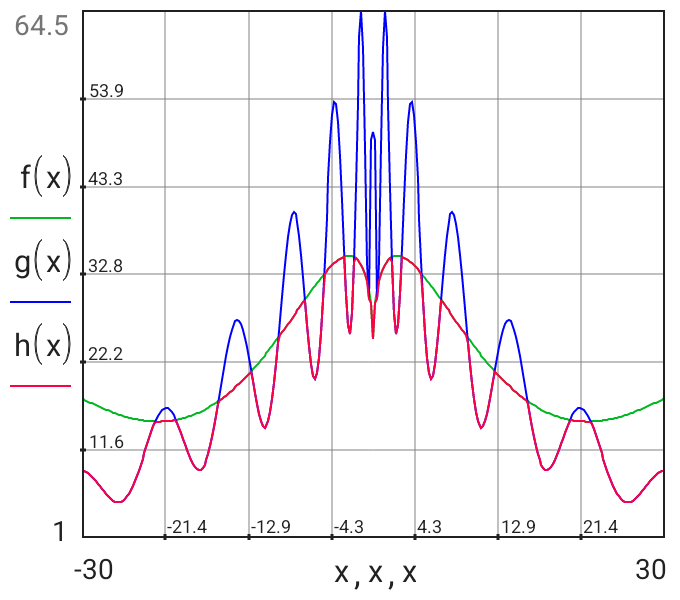
\includegraphics[width=0.45\textwidth]{graphics/function_plot_fig4.png} \end{tabular}\end{center}

Haciendo un largo toque en el centro
del área de la gráfica, aparecerá el
menú contextual y el botón flotante
''Propiedades de los objetos''.
\begin{center}\begin{tabular}{c} 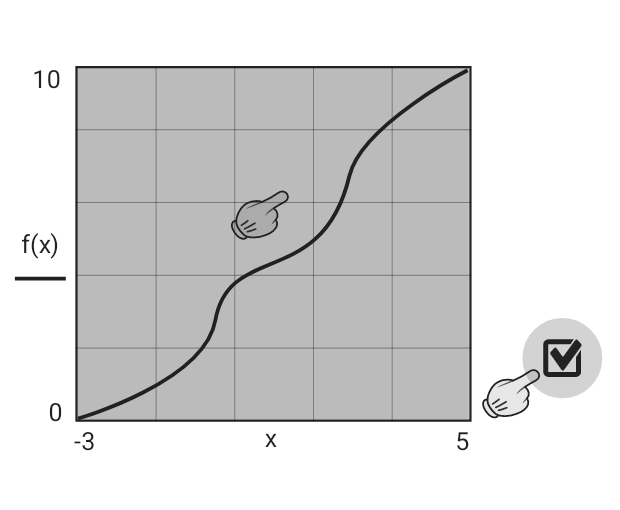
\includegraphics[width=0.45\textwidth]{graphics/function_plot_fig5.png} \end{tabular}\end{center}

Si presiona este botón flotante, se
mostará el diálogo de ''Ajustes de la
gráfica''. Aquí, puedes cambiar el
tamaño y el estilo del área de la
gráfica. Por ejemplo, el gráfico
cruzado se ve como esto:
\begin{center}\begin{tabular}{c} 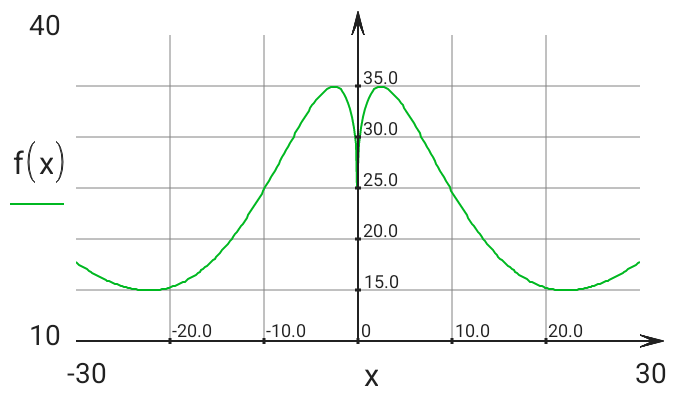
\includegraphics[width=0.45\textwidth]{graphics/function_plot_fig6.png} \end{tabular}\end{center}

También puedes cambiar la línea del
gráfico color, anchura y estilo en el
diálogo ''Ajustes de línea''. Aparece al
mantener presionado en la línea
marcada debajo del nombre de la
función a la izquierda de área de la
gráfica:
\begin{center}\begin{tabular}{c} 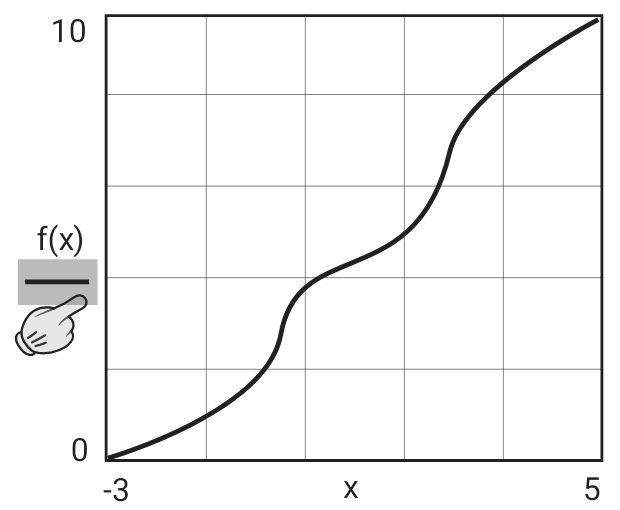
\includegraphics[width=0.45\textwidth]{graphics/function_plot_fig7.png} \end{tabular}\end{center}

Por ejemplo, podemos usar líneas
punteadas:
\begin{center}\begin{tabular}{c} 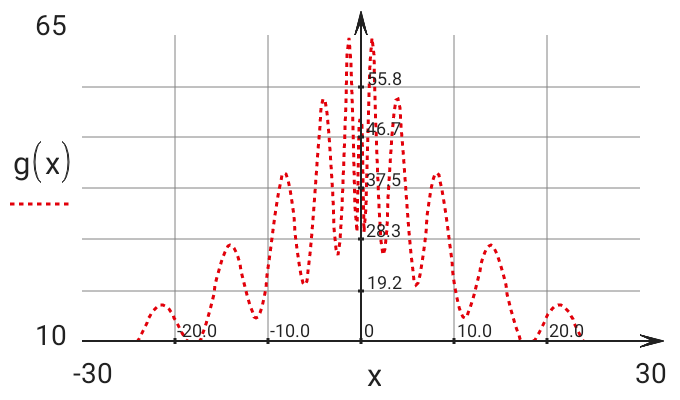
\includegraphics[width=0.45\textwidth]{graphics/function_plot_fig8.png} \end{tabular}\end{center}

El número de etiquetas de los ejes y la
línea de la cuadrícula color se puede
cambiar en el diálogo ''Ajustes de
cuadrícula''. Aparece al mantener
presionado en el espacio libre entre
el  valor mínimo de x (-30) y el
símbolo del argumento (x) o entre el
símbolo x junto al valor máximo x (30)
debajo del área de la gráfica
\begin{center}\begin{tabular}{c} 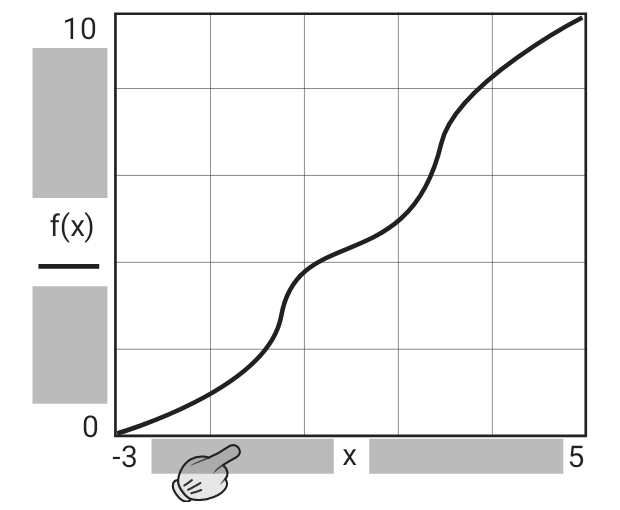
\includegraphics[width=0.45\textwidth]{graphics/function_plot_fig9.png} \end{tabular}\end{center}
\begin{center}\begin{tabular}{c} 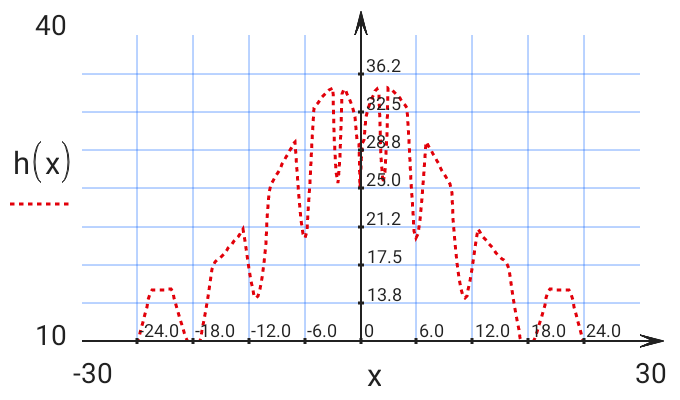
\includegraphics[width=0.45\textwidth]{graphics/function_plot_fig10.png} \end{tabular}\end{center}

Para ocultar la cuadrícula por completo
sólo hay que poner a cero el número de
líneas de la cuadrícula para ambos
ejes verticales y horizontales. Para
ocultar la cuadrícula por completo
sólo hay que poner a cero el número de
líneas de la cuadrícula para ambos
ejes verticales y horizontales.